\chapter{Theoretical Background}
\label{Introduction}
%
\epigraph{``\textit{You must understand, young Hobbit, it takes a long time to say anything in Old Entish. And we never say anything unless it is worth taking a long time to say.}"}{J.R.R. Tolkien}
%
This chapter presents a description of the two computational methods which have been primarily applied throughout the course of this thesis. Certain aspects of the thesis have required the use of other simulation methods, and these methods are outlined in the respective chapters.

\section{Molecular dynamics}\label{chapter:MD}
%
Molecular dynamics (MD) is a simulation method to study the dynamic evolution of a system of particles over time in accordance with their predefined interaction rules. For a macromolecular system, this is a powerful tool that is used to complement experiments to investigate the system to atomic resolution in space and \edit{femto}second resolution in time, to predict structural and thermodynamic properties such as free energies.\cite{mcquarrie1965statistical} The structural and thermodynamic behaviour can be compared to experimental data and provide insight to complex processes such as adsorption or ligand binding. An MD engine is a collection of numerical algorithms that defines a set of forces that act on all particles in a system, and iteratively evolves them along trajectories according to Newton's equations of motion.
%
\begin{equation} \label{eq:newtons2nd}
m_i \frac{\partial^2\mathbf{r}_i}{\partial t^2}=\mathbf{F}_i,\quad  i = 1,\,\dots,\,N
\end{equation}
%
Forces acting on particles $\mathbf{F}_i$ at positions $\mathbf{r}_i$ evolve the system to new positions according \edit{to} the potential energy function $U(\mathbf{r}_i$).
%
\begin{equation} \label{eq:newton}
\mathbf{F}_i = -\frac{\partial U}{\partial \mathbf{r}_i}
\end{equation}
%
In the case of biomolecular systems, the predefined interaction rules are a potential energy function (forcefield) which are requisite to calculating the forces. A forcefield maps the coordinates of the atoms $\mathbf{r}$ onto the potential energy surface as per the bonded and non-bonded energetic contributions of the macromolecular system components; namely the bonds, angles and dihedrals between atoms (bonded) and van der Waals and electrostatic (non-bonded) interactions.\cite{de2016role} A forcefield is usually expressed as sums of particle interactions and in the case of the \textit{optimised potentials for liquid simulations} (OPLS) forcefield \cite{jorgensen1988opls, jorgensen1996development} it takes the form expressed in (Eq.~\ref{eq:forcefield}), where ($K_b,\,K_{\theta},\,K_l,\,$) are respectively the bond, angle and dihedral force constants for each bonded interaction type and ($r_0,\, \theta_0,\, \phi_l$) are the equilibrium terms. The Lennard-Jones parameters ($\sigma_{ij}$,\, $\epsilon_{ij}$) that describe the interactions between types $i$ and $j$ are determined by taking a geometric average of the self-interaction parameters, i.e. ($(\sigma_{ii}\sigma_{jj})^{1/2}$). The final term in (Eq.~\ref{eq:forcefield}) is the Coulombic term that describes the energy between a pair of charges ($q_i,\,q_j$). 
%
\begin{equation} \label{eq:forcefield}
\begin{split}
U(\mathbf{r}) &= \sum_{bonds} K_b(r - r_0)^2 + \sum_{angles} K_{\theta}(\theta - \theta_0)^2 + \sum_{dihedrals} \, \, \sum_{l=1}^{4} \frac{K_{l}}{2}\left[1+(-1)^{l+1}\cos{(l\phi -\phi_{l})}\right] \\
&+ \sum_{nonbonded} 4\epsilon_{ij} \left[ \left( \frac{\sigma_{ij}}{r_{ij}}\right)^{12}-\,\,\left( \frac{\sigma_{ij}}{r_{ij}}\right)^{6} \right] + \sum_{i > j}  \frac{q_{i}q_{j}}{\edit{4 \pi \epsilon_{0}}r_{ij}}
\end{split}
\end{equation}
%
The principle of each bonded and non-bonded forcefield terms are illustrated in (Fig.~\ref{fig_ff}). Conventional potential energy functions describe a system with fixed charge for electrostatic interactions, electronic repulsion and dispersive non-bonded interactions through a van der Waals (Lennard-Jones) potential and bond stretching, bending and dihedral angle torsion potentials. More complex formulations of the potential energy function can include polarisation effects in polarisable forcefields,\cite{ponder2010current} or reactive forcefields that can account for bond order, bond formation and breaking.\cite{van2001reaxff}
%
\begin{figure}[H]
    \centering
    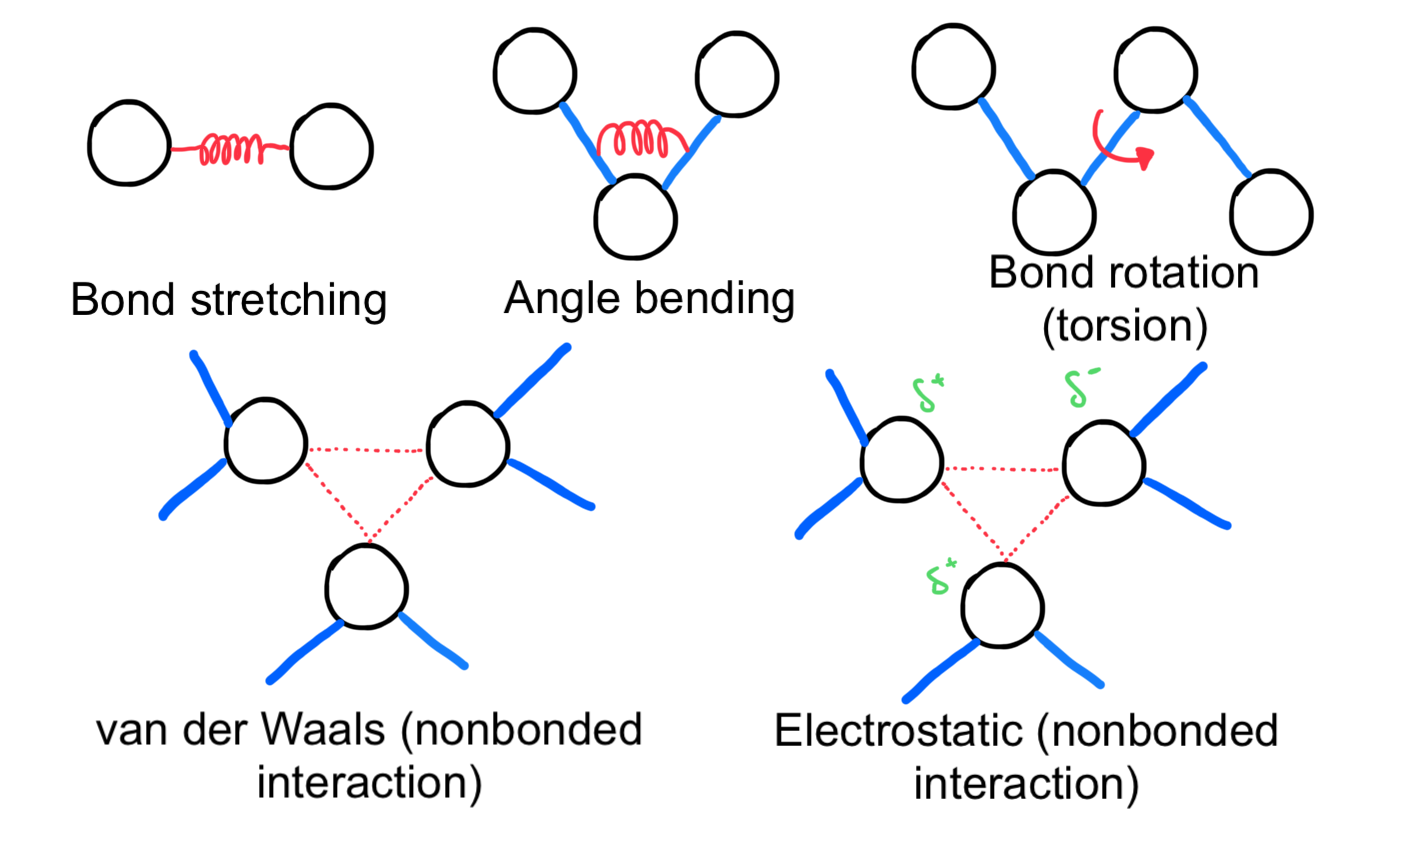
\includegraphics[width=0.99\columnwidth]{fig_ff.png}
    \caption{The energetic bonded and non-bonded components of a general biomolecular forcefield.}
    \label{fig_ff}
\end{figure}
%
The functional form of a forcefield (Eq.~\ref{eq:forcefield}) is composed of thousands of parameters for different types of atoms, bonds, bond angles, dihedral angles and nonbonded interactions.\cite{harder2016opls3} These parameters are typically derived semi-empirically through \textit{ab initio} quantum calculations on small molecules as well as optimising parameters to reproduce experimental properties of systems such as liquid densities and heats of vaporisation,\cite{vanommeslaeghe2010charmm} but retain the ability to accurately extrapolate to macromolecular properties such as the distribution of conformers such as $\phi,\, \psi$ angle distributions in proteins.\cite{mackerell2004improved} The transferability of forcefields is of course limited to the training and test sets, using them with an assumption of total coverage is erroneous, therefore special care is required when studying the dynamics of molecules with novel chemistries such as drug structures or exotic nanomaterials.\cite{harder2016opls3} One approach to derive the bespoke forcefield parameters from \textit{ab initio} quantum mechanical calculations is discussed in (\ref{sec:ddec}).
%
\subsection{Numerical integrators} \label{sec:integrators}
%
%\epigraph{``To do the same thing over and over again is not only boredom: it is to be controlled by rather than to control what you do."}{Heraclitus}
%
To solve \edit{the equations of motion (Eq.~\ref{eq:newtons2nd})} and translate the particle coordinates in the simulation system, one of many possible numerical integration methods is applied to approximate the exact solution to the differential equation. These methods generally start by replacing the derivative with a finite difference approximation of the form (Eq.~\ref{eq:finitediff}). 
%To solve a first order differential equation such as the one in (Eq.~\ref{eq:newton}) and translate the particle coordinates in the simulation system, one of many possible numerical integration methods is applied to approximate the exact solution to the differential equation. These methods generally start by replacing the derivative with a finite difference approximation of the form (Eq.~\ref{eq:finitediff}). 
%
\begin{equation} \label{eq:finitediff}
    \mathbf{r}'(t) \approx \frac{\mathbf{r}(t+\mathrm{d}t) - \mathbf{r}(t)}{\mathrm{d}t}
\end{equation}
This is rearranged to approximate new particle coordinates according to the force (Eq.~\ref{eq:newton}) and potential energy function (Eq.~\ref{eq:forcefield}), with respect to a discretised timestep $\mathrm{d}t$, this is known as the forward Euler algorithm (Eq.~\ref{eq:euler}).
%
\begin{subequations} \label{eq:euler}
%\begin{eqnarray}
\begin{align}
\begin{split}
    \mathbf{r}_i(t+\mathrm{d}t) &=  \mathbf{r}_i(t) +  \mathbf{v}_i(t)\mathrm{d}t
\end{split}\\
\begin{split}
    \mathbf{v}_i(t+\mathrm{d}t) &=  \mathbf{v}_i(t) + \frac{\mathbf{F}_i(\{\mathbf{r}_i(t)\})}{m_i}\mathrm{d}t
\end{split}
\end{align}
%\end{eqnarray}
\end{subequations}
%
This approach is first order convergent, meaning it has a local truncation error $\epsilon_{t+\mathrm{d}t}$ of order 2; namely the difference between the analytical ($\mathbf{r}(t+\mathrm{d}t)$) and approximated ($\mathbf{\tilde{r}}(t+\mathrm{d}t)$) solutions:
\begin{equation}
    \epsilon_{\,t+\dt} = \left|\mathbf{r}(t+\dt) - \mathbf{\tilde{r}}(t+\dt)\right|
\end{equation}
The analytical solution is expressed as a truncated Taylor series expansion:
\begin{equation}
    \mathbf{r}(t+\dt) = \mathbf{r}(t) + \mathbf{r'}(t)\dt + \frac{1}{2}\mathbf{r''}(t)\dt^2 %+ \frac{1}{6}\mathbf{r'''}(t)\dt^3
\end{equation}
Such that the truncated error of a single integration step using the forward Euler algorithm is given by:
\begin{subequations} \label{eq:euler_error}
%\begin{eqnarray}
\begin{align}
\begin{split}
    \epsilon_{\,t+\dt} &= \left|\mathbf{r}(t+\dt) - \mathbf{\tilde{r}}(t+\dt)\right|
\end{split}\\
\begin{split}
    &=  \left|\mathbf{r}(t) + \mathbf{r'}(t)\dt + \frac{1}{2}\mathbf{r''}(t)\dt^2 - \left[   \mathbf{r}(t) + \mathbf{v}(t)\dt   \right]\right|
\end{split}\\
\begin{split}
    &= \left| \frac{1}{2} \mathbf{r''}(t)\dt^2 \right| = \mathcal{O}(\dt^2)
\end{split}
\end{align}
%\end{eqnarray}
\end{subequations}
\vspace{-0.1cm}
As the integrator evolves the system coordinates iteratively, this error accumulates with respect to the size of the time step $\dt$, a scenario where the numerical solution converges to the analytical solution is therefore only possible in the limit of $\dt \rightarrow 0$, which is an impractical obstacle that would stand in the way of simulating meaningful (long enough) trajectories. The accumulation of errors results in the gradual change of the total energy of a closed system over time, an artefact known as energy drift. To accurately model the dynamics of a system at equilibrium, integrators are required to be symplectic, have time reversible symmetry and conserve linear momentum, angular momentum and energy. The forward Euler algorithm breaks both time-reversible symmetry i.e. whether the model is invariant to the substitution $\dt \rightarrow -\dt$, and symplectic condition i.e. that phase space volume is conserved. 

The leapfrog algorithm overcomes these limitations by performing a half velocity update step, followed by a full position update. New positions are used as initial conditions for computing a new set of atomic forces, combined with the final velocity half step this gives the velocity at the full step (Eq.~\ref{eq:froggy}).  
\begin{subequations} \label{eq:froggy}
%\begin{eqnarray}
\begin{align}
\begin{split}
\mathbf{v}_{i} \left(t + \frac{\dt}{2}\right) &= \textbf{v}_{i} (t) + \frac{\mathbf{F}_i(\{\mathbf{r}_i(t)\})}{m_i}\frac{\dt}{2} 
\end{split}\\
\begin{split}
\mathbf{r}_{i} (t + \dt) &= \mathbf{r}_{i} (t) + \mathbf{v}_{i} \left(t + \frac{\dt}{2}\right)\dt
\end{split}\\
\begin{split}
\mathbf{v}_{i} (t + \dt) &= \textbf{v}_{i} \left(t + \frac{\dt}{2}\right) + \frac{\mathbf{F}_i(\{\mathbf{r}_i(t+\dt)\})}{m_i}\frac{\dt}{2}
\end{split}
\end{align}
%\end{eqnarray}
\end{subequations}
The leapfrog algorithm is second order convergent and therefore has a local truncation error of order 3, following the same approach in (Eq.~\ref{eq:euler_error}):
\begin{subequations} \label{eq:froggy_error}
%\begin{eqnarray}
\begin{align}
\begin{split}
    \epsilon_{\,t+\dt} &= \left|\mathbf{r}(t+\dt) - \mathbf{\tilde{r}}(t+\dt)\right|
\end{split}\\
\begin{split}
    &= \left| \frac{1}{6} \mathbf{r'''}(t)\dt^3 \right| = \mathcal{O}(\dt^3)
\end{split}
\end{align}
\end{subequations}
The leapfrog algorithm (Eq.~\ref{eq:froggy}) meets the conditions outlined above and does not give rise to numerical artefacts for long simulation times as with the forward Euler algorithm. 

\subsection{Initial configuration} 
%
The investigation of a system's dynamics using an MD engine --- employing the algorithms covered in this chapter --- requires the user to identify molecular constituent atom types, atomic coordinates, the topology of the molecules of interest and their velocities. The input system structure is recognised by the employed forcefield to assign parameters in accordance with the functional form of the forcefield, generalised by (Eq.~\ref{eq:forcefield}). 

The user defined input coordinates of the system are paramount to correctly modelling the physical body under investigation; whether a protein, ligands or nanomaterials, it can be experimentally derived or inferred but requires pre-processing to ensure no experimental or modelling errors are present. Protein structures are available from X-Ray Diffraction (XRD) experiments, in the form of crystallographic 3-dimensional coordinate data hosted on the protein data bank (PDB) archive.\cite{PDB} A common experimental artefact from PDB structures is missing residues in the amino acid sequence, these are remedied using homology modelling. MODELLER is such a program, it performs comparative protein structure modelling by satisfaction of spatial restraints, filling in missing residues by aligning the input protein amino acid sequence to known related structures, producing 3-dimensional protein structures.\cite{marti2000comparative, webb2016comparative} 

In the case of small molecules such as ligands, widely available software packages can be utilised to define the input structure of molecules by hand using an interactive interface such as Avogadro.\cite{hanwell2012avogadro} Meanwhile, large non-organic materials can be generated by one of the many functionalities of the more complex initial configuration generators such as CHARMM-GUI; a web-hosted graphical user interface with an extensive set of tools ranging from nanomaterial, polymer and lipid membrane builders with multi-forcefield and multi-MD engine support.\cite{jo2008charmm,Lee2020} Another example of a versatile initial configuration builder is Packmol, it is a script-based and locally hosted software package that is widely used for generating complex systems.\cite{martinez2009packmol} Packmol affords user flexibility in ways interactive software may not, such as building the initial configuration of systems composed of different constituent molecules.

For entirely bespoke systems the molecular configuration is inferred through experimental techniques that do not accurately translate to 3-dimensional coordinates as is the case with proteins from the PDB. In particular, systems with exotic chemistries are not always readily prepared using the aforementioned initial configuration software, beside standardised protocol that may not reflect the accurate theoretical/phenomenological structure of the system in question. Such systems would require accuracy both in the distribution of atoms within the macromolecule as well as assigning the correct forcefield parameters. For example, some of the work in this thesis required the accurate characterisation of graphitic nanomaterials that required custom software to develop the macromolecular structures, topological properties and their corresponding forcefield parameters.\cite{albadri2020accurate-github} Custom software allows for flexibility in varying nanomaterial structural properties such as shape, size, chemical functionalisation and degree of functional group correlation. Software engineering custom software is an incredibly time consuming project, which is being accelerated by well executed and documented open source software initiatives.

\subsection{Periodic boundary conditions}
Periodic boundary conditions (PBC) are imposed on most MD simulation systems to approximate large systems that reside in a practically infinite environment, by construction. Simply put, particles leaving the unit cell in any of the ($\mathbf{x,y,z}$) directions reenter the unit cell from the opposing side in the respective dimension, retaining identical mechanical properties such as particle momenta. Particles in the unit cell interact with the particles in the closest neighbouring unit cell, restricted by the interaction cut-off radius as input by the user. As is common\edit{ly} the case and has been explained, the initial configuration can raise simulation artefacts and PBCs are no exception. A macromolecule such as a protein can self-interact through the boundary conditions, resulting in distorted dynamics if and when the simulation system is too small and the macromolecule isn't enveloped by sufficient explicit solvent molecules in all of the ($\mathbf{x,y,z}$) directions. The recommended protocol is that the simulation system should exceed twice the cut-off radius and have at least 1 nm of explicit solvent surrounding the macromolecule.\cite{deSouza1997} Charge interactions through PBCs could raise electrostatic artefacts, where a system without a neutral charge could sum to infinite charge through the periodic cells. Instead counter-ions are added to bring the simulation system to neutral charge, usually this sodium and chlorine ions for positive and negative charges, respectively. 

\subsection{Equilibration} \label{sec:equilibration}
The software used to create the initial configuration does not typically consider the energetics of the system, it is instead more suited to successfully geometrically organise a system's 3-dimensional molecular coordinates. As a result, these configurations may --- according to the initial configuration method --- exist in a high energy state, driven by anything from a high degree of atomic overlap to energetically unfavourable molecular conformations. Studying the system at equilibrium therefore requires a sequential treatment to bring the system's potential energy to a local minimum, followed by simulating trajectories to bring about thermal and barostatic equilibrium. These are known as the equilibration steps that precede the so called production-run which is used to gather the statistics for the desired system. 

\subsubsection{Energy minimisation}
To overcome the high energy of the initial configuration of the system, the MD engine employs the chosen forcefield to tweak the system coordinates until the energy corresponds to a local minimum in the potential energy surface through energy minimisation, instead of employing MD algorithms. A common approach to locate the local minimum of a multivariate and highly dimensional function that cannot be solved analytically is the gradient descent algorithm. A parameter (coordinate) vector ($\mathbf{r}$) is iteratively updated in the negative direction to the first order local gradient of the function ($\nabla \,V(\mathbf{r})$) being minimised in accordance with (Eq.~\ref{eq:gradient_descent}) until reaching convergence when the gradient is zero. The gradient is scaled by the step size ($\eta$), also known as the learning rate, the choice of which can impact whether the algorithm reaches convergence. Too small a step size could significantly retard the convergence, whereas a large step size could overshoot the local minimum parameter vector. 
%
\begin{equation} \label{eq:gradient_descent}
    \mathbf{r}_{n+1} = \mathbf{r}_{n} - \eta_{n} \, \nabla \, V(\mathbf{r}_{n})
\end{equation}
%
Tweaking the step size is therefore paramount to effectively or efficiently locate a local minimum; one such approach is a particular case of gradient descent known as the steepest descent algorithm, where the step size ($\eta$) is iteratively chosen to maximise the direction of the negative gradient of the function by minimising the objective function (Eq.~\ref{eq:obj_func}).\cite{Curry1944} 
%
\begin{equation} \label{eq:obj_func}
    \eta_n = \argmin_{\eta} \, \, V ( \mathbf{r}_{n} - \eta \, \nabla \, V(\mathbf{r}_{n})) 
\end{equation}
%
\subsubsection{Particle velocities}
To model the system in equilibrium, the system potential energy should oscillate close to its local minimum due to fluctuations in kinetic energy. Ensuring these oscillations in potential energy are stable and do not diverge due to large fluctuations, initial velocities are assigned to every particle in the system. There exist statistical constraints on the choice of particle velocities to ensure the system is in thermal equilibrium, namely that it abides by the equipartition theorem. To abide by this, all particles are randomly assigned a velocity from the Maxwell-Boltzmann distribution given by (Eq.~\ref{eq:Maxwell_distro}), where ($v$) is the velocity magnitude ($\sqrt{v_x^2 + v_y^2 + v_z^2}$) of the velocity vector ($\mathbf{v} = (v_x, v_y, v_z)$) and ($m$), ($T$) and ($k_B$) are the mass, desired temperature and the Boltzmann constant, respectively. 
%
\begin{equation} \label{eq:Maxwell_distro}
    f(v) = \frac{4}{\sqrt{\pi}} \left( \frac{m}{2k_B T} \right)^{3/2} v^2 \, \exp{\left( - \frac{mv^2}{2k_B T}\right)}
\end{equation}
%
Using this, the average square velocity is given by the integral:
\begin{equation}
    \langle v^2 \rangle = \int_0^{\infty} v^2 f(v)\,\mathrm{d}v = \frac{3k_B T}{m}
\end{equation}
%
%\subsection{Constraint algorithms}
%The application of numerical integrators as discussed in section (\ref{sec:integrators}) can be made more efficient by extending the rate of integration (update step) in (Eq.~\ref{eq:froggy}) without encroaching on the time-frequency of the fastest dynamics in the simulation system. It turns out that the highest frequency dynamics in any biomolecular system is the bond frequency of the 
%\subsubsection{LINCS}

\subsection{Thermostats}
%
%\epigraph{``The worst thing you can do about a situation is nothing."}{Ice Cube}
%
Performing iterative integration of Newton's equations of motion (Eq.~\ref{eq:newton}) in this way generates a microcanonical ensemble where the simulation system's number of atoms ($N$), volume ($V$) and total energy ($E$) are kept constant. With conserved energy, the system is in a steady state that does not evolve over time, despite all its constituent parts being in motion. The microcanonical ($NVE$) ensemble assigns equal probability to all the system microstates within this energy $E$, all microstates outside this range have zero probability and are never sampled in an equilibrium configuration. The alternative approach is to model the system in a canonical ($NVT$) ensemble, where the system no longer has conserved energy but the average temperature ($T$) is kept constant. By allowing the simulation system to exchange energy with its environment --- implemented through coupling to a heat reservoir --- it is able to explore a phase space that includes microstates with different energies.\cite{ford2013statistical} In order to implement the canonical ensemble in MD simulations, in which temperature is conserved instead of energy, the integration of Newton's equations of motion have to be coupled to a thermostat. 

A thermostat is an algorithm that introduces a fictitious dynamical variable, which slows down or accelerates particles until the temperature is equal to the desired value through coupling to an external heat bath. One of the simplest implementations of a thermostat is the Berendsen thermostat which rescales the velocities of all particles at each integrator timestep with a nonphysical force (Eq.~\ref{eq:berendsen}) with a scale factor ($\lambda$) to control the total mean kinetic energy.\cite{berendsen1984molecular} 
%
\begin{equation} \label{eq:berendsen}
    \lambda\,(t) = \left[    1 + \frac{\dt}{\tau_{\,T}} \left( \frac{T_0}{T(t-\frac{1}{2}\dt) - 1}   \right) \right]^{1/2}
\end{equation}
%
$\tau$ is a time constant related to the temperature coupling time constant $\tau_T$ by $\tau = 2C_V \tau_T / N_{df}k_B$, where $C_V$ is the total heat capacity of the system, $N_{df}$ the numer of degrees of freedom in the system and $k_B$ is the Boltzmann constant. Deviations of the simulation system temperature $T_0$ are corrected to the target temperature $T$ according to:
\begin{equation} \label{eq:berendsen_rate}
    \frac{\mathrm{d}T}{\dt}  = \frac{T_0 - T}{\tau}
\end{equation}
%
The system kinetic energy ($K$) is scaled with $\lambda$ (Eq.~\ref{eq:berendsen}) at each integrator step through:
\begin{equation} \label{eq:berendsen_kinetic}
    \Delta\, K = (\lambda - 1)^2\, K
\end{equation}

By design (see \ref{sec:equilibration}) the particle velocities are distributed according to the Maxwell-Boltzmann function. Scaling the kinetic energy with the Berendsen thermostat (Eq.~\ref{eq:berendsen_kinetic}) suppresses the fluctuations in kinetic energy and particle velocities no longer adopt a Maxwell-Boltzmann distribution. This means that the Berendsen thermostat does not generate a canonical ensemble and will give rise to artefacts and incorrect sampling of the system's phase space. A particular manifestation within a system is that the total kinetic energy is not shared equally among all kinetic degrees of freedom --- hence violating the theory of equipartition --- where the kinetic energy instead flows from higher energy degrees of freedom to translational and rotational degrees of freedom. This results in a part of the system freezing into a single conformation and travelling through the simulation box with high momentum, this is known as the flying ice cube effect.\cite{harvey1998flying} 

To remedy this artefact, a stochastic term ($\mathrm{d}W$) in the form of a Wiener process is added to the Berendsen thermostat (Eq.~\ref{eq:berendsen}) that ensures the correct kinetic energy distribution and that the resulting dynamics produce a correct canonical ensemble.
%
\begin{equation} \label{eq:bussi_thermostat}
    \mathrm{d}K = (K_0 - K)\frac{\dt}{\tau_{\,T}} + 2 \sqrt{\frac{K\,K_0}{N_{df}}} \frac{\mathrm{d}W}{\sqrt{\tau_{\,T}}}
\end{equation}
This is known as the Bussi–Donadio–Parrinello thermostat (Eq.~\ref{eq:bussi_thermostat}).\cite{bussi2007canonical}
\subsection{Barostats}
In a similar fashion, an isothermal-isobaric ($NPT$) ensemble can be generated by a rigorous barostat algorithm by coupling the system to a pressure bath. One approach that successfully generates an isothermal-isobaric ensemble is the Parinello-Rahman barostat.\cite{parrinello1981polymorphic} This approach is implemented through coupling the imbalance between the simulation system pressure and the external (bath) tensorial pressure field to changes in the shape and size of the simulation box. The simulation box vectors are represented by the matrix ($\mathbf{b}$) and obey the equation of motion in (Eq.~\ref{eq:PR_EoM}), defined with respect to the simulation box volume ($V$), coupling strength matrix ($\mathbf{W}$), system pressure ($\mathbf{P}$) and reference pressure ($\mathbf{P}_{ref}$).
%
\begin{equation} \label{eq:PR_EoM}
    \frac{\mathrm{d}\mathbf{b}^2}{\dt} = V \mathbf{W^{-1}}\mathbf{b'}^{-1} (\mathbf{P}-\mathbf{P}_{ref})
\end{equation}
%
The system pressure tensor ($\mathbf{P}$) is calculated from the difference in kinetic energy ($\mathbf{K}$) and the virial tensors (Eq.~\ref{eq:virial}), where ($\otimes$) denotes the tensor product. 
%The scalar pressure is calculated from the pressure tensor through $P = \mathrm{Tr}(\mathbf{P})/3$. 
%
\begin{subequations} \label{eq:virial}
%\begin{eqnarray}
\begin{align}
\begin{split}
    \mathbf{P} = \frac{2}{V}(\mathbf{K} - \Xi)
\end{split}\\
\begin{split}
    \mathbf{K} = \frac{1}{2}\sum_i m_i \mathbf{v}_i \otimes \mathbf{v}_i
\end{split}\\
\begin{split}
    \Xi = -\frac{1}{2}\sum_{i<j} \mathbf{r}_{ij} \otimes \mathbf{F}_{ij} 
\end{split}
\end{align}
\end{subequations}
% if you want derivations and more special cases (PBC) see https://cfwebprod.sandia.gov/cfdocs/CompResearch/docs/JCPSA613115154107_1.pdf
%
The coupling strength matrix ($\mathbf{W}$) is defined with respect to the isothermal compressibility ($\beta_{ij}$), pressure time constant ($\tau_P$) and the largest box matrix element ($L$) as $(\mathbf{W}^{-1})_{ij} = 4 \pi^2 \beta_{ij} / 3 \tau_P^2 L$. Since the implementation of pressure coupling requires a change in both simulation box vector and particle equations of motion, a modification is applied to the system Hamiltonian, where the modified Hamiltonian ($\mathcal{H}_{PR}$) is given by (Eq.~\ref{eq:PR_hamil}), where ($U$) and ($K$) denote the potential and kinetic energies, respectively. 

\begin{equation} \label{eq:PR_hamil}
    \mathcal{H}_{PR} = U + K + \sum_i P_{ii} V + \sum_{ij} \frac{1}{2} W_{ij} \left(\frac{\mathrm{d}\,b_{ij}}{\dt}\right)^2
\end{equation}

The equations of motion of the system's particles are given by (Eq.~\ref{eq:PR_motion}), where the added term takes the form of a friction term. It is however fictitious and solely there to define the particle equations of motion with respect to the simulation box vectors through the term.

\begin{subequations} \label{eq:PR_motion}
%\begin{eqnarray}
\begin{align}
\begin{split}
    \frac{\mathrm{d}^2 \mathbf{r}_i}{\dt^2} = \frac{\mathbf{F}_i}{m_i} - \Lambda \frac{\mathrm{d} \mathbf{r}_i}{\dt}
\end{split}\\
\begin{split}
    \Lambda = \mathbf{b}^{-1} \left[  \mathbf{b} \frac{\mathrm{d}\mathbf{b'}}{\dt} + \frac{\mathrm{d}\mathbf{b}}{\dt} \mathbf{b'} \right] \mathbf{b'}^{-1}
\end{split}
\end{align}
\end{subequations}
%
\subsection{Parallelisation}
Simulating the dynamics of biomolecular systems requires a large system size to answer questions of meaningful scientific interest. The computational cost of running MD algorithms scales with the number of particles in the simulation system, therefore the implementation of MD algorithms in parallelised standards is necessary. Accelerating MD simulations is achieved by both parallelised standards where the software code is written to specify how tasks are divided between computational resources, and by implementing methods that reduce the complexity of particularly costly calculations involved in MD algorithms, e.g. evaluating a list of distances between particles and calculating long-range interactions. 

\subsubsection{Domain decomposition}
The naive approach of calculating the distances between particle coordinates in the simulation system is through a brute-force algorithm, where the distances are computed between all ($N(N-1)/2$) point pairs and the smallest distance pair is picked. The list of distances is used to evaluate the interaction type and its magnitude, thus its contribution to the total system energy at that point in the simulation. Performing this by brute force requires $\mathcal{O} (N^2)$ time. An alternative approach to calculating particle pair-wise distances and their interactions is known as domain decomposition, in which a data structure is implemented where distances are evaluated only within a predefined cut-off distance, therefore reducing the $\mathcal{O} (N^2)$ time complexity of the closest pair of points problem. The cut-off distance is generally the distance within which short-range non-bonded interactions are present. This data structure works by decomposing the 3-dimensional simulation domain into cells with a edge length equal to or greater than the interaction cut off distance, where pairwise distances are now computed for particles between neighbouring cells instead of the entire simulation domain. For a 3-dimensional simulation domain, a 3-dimensional cell has 26 neighbouring cells for which pairwise distances need to be calculated. The computational time complexity of this operation is reduced from $\mathcal{O} (N^2)$ to $\mathcal{O} (N\overline{c}) \in \mathcal{O} (N)$, where $\overline{c}$ denotes the average number of particles per cell ($N/m$), where ($m$) is the number of cells decomposing the domain. 

\subsubsection{Particle-mesh-Ewald summation} \label{sec:pme}
Having reduced the cost of evaluating particle pairwise distances for short-range interactions does not solve the problem of computing pairwise distances to calculate long range non-bonded interactions, such as electrostatics and the Lennard-Jones dispersion ($1/r^6$) term in (Eq.~\ref{eq:forcefield}). Ewald summation \cite{ewald1921berechnung} was introduced for the treatment of such long-range interactions, however it scales as ($\mathcal{O}(N^2)$) in time which is impractical for the treatment of large simulation systems. However it does form the foundations of methods such as particle-mesh-Ewald (PME) \cite{Darden1993} which scales as ($\mathcal{O}(N\,\log\,N)$) in time.

Within Ewald summation formalism, the total electrostatic energy for $N$ particles for a unit cell --- defined with respect to periodic images at positions ($\mathbf{r}_j + \mathbf{n}$) --- is represented by (Eq.~\ref{eq:ewald_unit_cell}), where ($\mathbf{n} =  n_1\mathbf{a}_1 + n_2\mathbf{a}_2 + n_3\mathbf{a}_3$) are the box index vectors and the ($\sum_{n}^{\ast}$) sum indicates that terms with ($i=j$) and ($\mathbf{n} = 0$) should be omitted. 
%
\begin{equation} \label{eq:ewald_unit_cell}
E(\mathbf{r}) = \frac{1}{2}\sum_{n}^{\ast}\sum_{i} \sum_{j} \frac{q_i q_j}{{\left| \mathbf{r}_j - \mathbf{r}_i + \mathbf{n} \right| }}
\end{equation}
%
The expression is a slowly converging sum that can be converted to quickly converging expressions for short-range ($E_{sr}$) and long-range ($E_{lr}$) electrostatic interactions and a self-interaction correction term ($E_{corr}$); long-range interactions are computed in reciprocal space through the use of Fourier transforms. \cite{ewald1921berechnung, Essmann1995}
%
\begin{subequations} \label{eq:ewald_sep}
\begin{align}
\begin{split}
E = E_{sr} + E_{lr} + E_{corr} 
\end{split}\\
\begin{split} \label{eq:ewald_sr}
E_{sr} = \frac{1}{2} \sum_{n}^{\ast} \sum_{i,j}^{N}  q_i q_j \frac{\mbox{erfc}\left(\beta \left| \mathbf{r}_j - \mathbf{r}_i + \mathbf{n} \right|\right)}{\left| \mathbf{r}_j - \mathbf{r}_i + \mathbf{n} \right|}
\end{split}\\
\begin{split} \label{eq:ewald_lr}
E_{lr} = \frac{1}{2 \pi V} \sum_{\mathbf{m} \neq 0} \frac{ \exp{(- \pi^2 \mathbf{m}^2 / \beta^2)}}{\mathbf{m}^2} S(\mathbf{m}) S(-\mathbf{m})
\end{split}\\
\begin{split} \label{eq:ewald_corr}
E_{corr}=-\frac{1}{2} \sum_{(i, j) \in M} \frac{q_{i} q_{j} \operatorname{erf}\left(\beta\left|\mathbf{r}_{i}-\mathbf{r}_{j}\right|\right)}{\left|\mathbf{r}_{i}-\mathbf{r}_{j}\right|}-\frac{\beta}{\sqrt{\pi}} \sum_{i}^{N} q_{i}^{2}
\end{split}
\end{align}
\end{subequations}
%
In (Eq.~\ref{eq:ewald_lr}), the volume of the unit cell ($V$) is given by ($\mathbf{a}_1 \cdot \mathbf{a}_2 \times \mathbf{a}_3$), ($\mathbf{m}$) denotes the reciprocal lattice space vectors ($\mathbf{m}  =  m_1\mathbf{a}_1^{\ast} + m_2\mathbf{a}_2^{\ast} + m_3\mathbf{a}_3^{\ast}$) and ($S(\mathbf{m}) = \sum_{j}^{N} q_j \exp{(2 \pi i\, \mathbf{m\cdot r})}$) is the structure factor. The error function ($\mathrm{erf}(x)$) in (Eq.~\ref{eq:ewald_corr}) is related to the complementary error function in (Eq.~\ref{eq:ewald_sr}) by ($1 - \mathrm{erfc}(x)$). The ($\beta$) parameter in (Eq.~\ref{eq:ewald_sep}) determines the relative weight of the direct and reciprocal sums and can be used to control the rates of convergence of the respective terms. Algorithmic optimisation of the ($\beta$) parameter can reduce the time complexity of Ewald summation from ($\mathcal{O}(N^2)$) to ($\mathcal{O}(N^{3/2})$).\cite{karasawa1989acceleration,Darden1993} 

The PME method also separates the short- and long-range interactions, similarly to the Ewald method in (Eq.~\ref{eq:ewald_sep}), where short-range and long-range interactions are evaluated in real and reciprocal space, respectively. The real space (short-range) sum has a time complexity of ($\mathcal{O}(N)$) by virtue of the pairwise minimum distance computation from domain decomposition, leaving the reciprocal space sum (Eq.~\ref{eq:ewald_lr}) as the bottleneck. The treatment of the long-range non-bonded interactions is accelerated to ($\mathcal{O}(N \log N)$) time complexity by assigning the charges ($q$) to a discrete grid (mesh) using cardinal B-spline interpolation, \cite{Essmann1995} resulting in a charge density field. The charge density field is defined on a discrete lattice in real space and is Fourier transformed to reciprocal space, enabling the long-range interaction term to be evaluated using a single sum over the grid in reciprocal ($\mathbf{k}$) space (Eq.~\ref{eq:pme}), where ($\tilde{\Phi}_{lr}(\mathbf{k})$) denotes the Fourier transformed potential from Ewald summation --- implicit in (Eq.~\ref{eq:ewald_lr}) --- and $\tilde{\rho}(\mathbf{k})$ the Fourier transformed charge density field.
%
\begin{equation} \label{eq:pme}
    E_{lr} = \sum_{\mathbf{k}} \tilde{\Phi}_{lr}(\mathbf{k}) \left| \tilde{\rho}(\mathbf{k})\right|^2  
\end{equation}
%
%
%\edit{Should I say something about how they're computationally implemented and how that helps with the parallelisation of MD algorithms, in line with the name of this chapter? --- CDL I think that would be nice}
%
%The evolution of high performance computing scale and their different architectures have had a big impact on the acceleration of MD simulations in recent decades, most notably the transferability between graphical processing unit (GPU) architecture and MD spatial domains. \edit{You would have to say more about this... cite implementation paper of gmx 2020 where all bonded and non-bonded interactions happen on GPU.} Other more bespoke architectures designed particularly for solving MD algorithms are at the cutting edge; simulating larger systems in a relatively short time. \edit{ANTON is ...} 
%\subsubsection{Domain decomposition}
%Within computational processing unit (CPU) parallelisation, a simulation system is divided by the number of CPU threads, such that --- at least in principle --- $N$ threads accelerate the simulation by $N$ times. Decomposing the simulation system into cells with respect to its coordinate Cartesian space by the available number of CPU threads is known as domain decomposition. In domain decomposition, integration algorithms are performed independently on each thread, while memory of neighbouring cells and their containing particles is maintained.
% ---------------------
%
%       DFT INTRO
%
% ---------------------
%\newpage
\section{Density Functional Theory} \label{chapter:onetep}
So far the discussion of molecular dynamics has considered the energetics and the calculation of forces on individual atoms in a macromolecular system, using Newton's  laws of motion in classical mechanics (Eq.~\ref{eq:newtons2nd}). The computation of energies and forces in classical MD is hinged on the validity of a forcefield that is derived from both \textit{ab initio} and phenomenological approaches. \textit{Ab initio} quantum mechanical approaches such as density functional theory (DFT) calculate the electronic ground state of a molecular system using the Schr\"odinger equation (Eq.~\ref{eq:schrodinger}) as a basis for its framework, which involves the treatment of both electrons and nuclei. Within the Schr\"odinger equation, the Hamiltonian operator ($\mathcal{H}$) acts on the quantum mechanical system; formulated in terms of the many electron wave function ($\Psi$).\cite{Schrodinger1926undulatory}
%
\begin{equation} \label{eq:schrodinger}
    \mathcal{\hat{H}}\, | \Psi \rangle = E \, | \Psi \rangle
\end{equation}
%
Solving the Schr\"odinger equation for a many electron system is an intractable and impossible problem to solve analytically, due to the correlated motion of electrons described by the many electron wave function ($\Psi$), containing $3N$ degrees of freedom, where $N$ is the number of electrons in question. DFT reformulates the Schr\"odinger equation from a single $N$-body problem to $N$ single-body problems.

Instead of the wave function, DFT solves the electronic Hamiltonian (Eq.~\ref{eq:molhamil}) by considering the density of the electrons in a system as a fundamental variable. It is expressed with respect to the kinetic energy operators for each electron ($\hat{T}_e$) and nucleus ($\hat{T}_e$) in the system, as well as the potential energy operators between the electrons and nuclei ($\hat{V}_{ne}$), electron-electron repulsion ($\hat{V}_{ee}$) and nuclei-nuclei repulsion ($\hat{V}_{nn}$). 
%
\begin{equation} \label{eq:molhamil}
\begin{split}
\hat{\mathcal{H}}  &=  \hat{T}_e + \hat{V}_{ne} + \hat{V}_{ee} + \hat{T}_{n} + \hat{V}_{nn}
\\ &= - \frac{\hbar}{2m} \sum_{i}^{N} \nabla_i - e^2 \sum_{I=1}^{N} \sum_{i=1}^{N} \frac{Z_I}{|\mathbf{R_I - r_i}|}  + \frac{e^2}{2} \sum_{i \neq j}^{N} \sum_{j \neq i}^{N} \frac{1}{|\mathbf{r_i - r_j}|} - \frac{\hbar^2}{2} \sum_{I=1}^{P} \frac{\nabla_i^2}{M_I} \\
& \quad + \frac{e^2}{2} \sum_{I=1}^{P} \sum_{J \neq I}^{P} \frac{Z_I Z_J}{|\mathbf{R_I - R_J}|}
\end{split}
\end{equation} 
%
The reformulation from wave functions to the density of electrons is based on Hohenberg-Kohn theorem and the Kohn-Sham equations. Fermi and Thomas first proposed this idea and derived a differential equation for the density,\cite{Thomas1927, fermi1927metodo} therefore negating the need to work in terms of the one-electron orbital. It later required the work of Hohenberg and Kohn to formulate the theory on a strong mathematical basis,\cite{hohkohn} giving rise to the Hohenberg-Kohn theorem. The theory was further developed with the Kohn-Sham framework,\cite{kohnsham} where the problem of interacting electrons in a static external potential is reduced to non-interacting electrons moving in an effective potential. 
%
The Born-Oppenheimer approximation makes solving the Schr\"odinger equation easier by imposing the separation of nuclear and electronic motion to the wave function ($\Psi(\mathbf{r}, \mathbf{R})$).\cite{BO} This is justified by the difference in momentum of the nuclei compared to electrons, where the much heavier nucle\edit{i} must therefore have minuscule velocities. 
%
\begin{equation} \label{eq:BO}
\Psi(\mathbf{r}, \mathbf{R}) = \psi(\mathbf{r}, \mathbf{R}) \phi(\mathbf{R})
\end{equation}
%
\subsection{Hohenberg-Kohn Theorems}
%
The Hohenberg-Kohn theorems are the basis for computing the ground state properties of a system without directly dealing with the highly dimensional many-electron wave function. It instead reformulates the problem in terms of the electronic density and treats the system of electrons moving under the influence of an external potential, which encompasses all effects external to the electrons themselves such as Coulombic effects from atomic nuclei. As such, and due to the separation of nuclear and electronic motion via the Born-Oppenheimer approximation, the repulsive Coulombic potential between nuclei can be treated separately as an external potential:
%
\begin{equation}
V_{\mathrm{ext}}(\mathbf{r})=-\sum_{I} \frac{Z_{I}}{\left|\mathbf{r}_I-\mathbf{r}_i\right|}
\end{equation}
%
Therefore the entire electronic Hamiltonian (Eq.~\ref{eq:molhamil}) can be expressed as ($\hat{H} = \hat{F} + \hat{V}_{\mathrm{ext}}$), where ($\hat{F}$) is given by (Eq.~\ref{eq:hohkohn_F}) and the external potential operator is given by the sum of external potentials ($\hat{V}_{\mathrm{ext}} = \sum_i V_{\mathrm{ext}} (\mathbf{r}_i)$).
%
\begin{equation} \label{eq:hohkohn_F}
\hat{F}=-\frac{1}{2} \sum_{i} \nabla_{i}^{2}+\frac{1}{2} \sum_{i} \sum_{j \neq i} \frac{1}{\left|\mathbf{r}_{i}-\mathbf{r}_{j}\right|} = \hat{T}_e + \hat{V}_{ee}
\end{equation}
%
The expression for ($\hat{F}$) is universal to all systems consisting of $N$ electrons, meaning that the external potential ($V_{\mathrm{ext}}$) and the number of electrons in a given system ($N$) completely control ($\hat{H}$) and the ground state wave function ($\Psi_0$). The ground state wave function and the Hamiltonian give rise to the ground state density ($n(\mathbf{r}$):
%
\begin{equation} \label{density}
n(\mathbf{r}) = \int \prod_{i=2}^{N} | \Psi_0 (\mathbf{r, r_2, r_3, \dots, r_N)}|^2 \mathrm{d} \mathbf{r}_i = \langle \Psi_0 | \hat{n} |\Psi_0 \rangle
\end{equation} 
%
Given this, the electronic density ($n(\mathbf{r})$) and the ground state wave function ($\Psi_0$) are functionals (a function of a function) of the number of electrons ($N$) and the external potential ($V_{\mathrm{ext}}$). 
 
The first Hohenberg-Kohn theorem states that the external potential ($V_{\mathrm{ext}}(\mathbf{r})$) is a unique functional of the ground state electronic density ($n(\mathbf{r})$), therefore the total energy is also a functional of the ground state electronic energy. Indeed, it turns out a consequence of this theorem is that all system properties can be determined just by the electronic ground state density.\cite{hohkohn} 

The proof for this theorem is a simple \textit{reductio ad absurdum} argument. Consider a many-electron Hamiltonian of the form ($H = T + V$) and a different Hamiltonian ($H' = T + V'$), with wave functions ($\Psi$) and ($\Psi '$) respectively and where ($V - V' \neq \mathrm{constant}$). The electron density is defined by (Eq.~\ref{density}) and we assume that the electron density is equal for ($V$) and ($V'$). 
%
According to the Rayleigh-Ritz variational theorem, the ground state energy satisfies the inequality (Eq.~\ref{ritz}).
%
\begin{subequations} \label{ritz}
\begin{align}
\begin{split}
E_0 < \langle \Psi'|H|\Psi'\rangle &= \langle \Psi'|H'|\Psi'\rangle + \langle \Psi'|H-H'|\Psi'\rangle
\end{split}\\
\begin{split}
&= E_0 ' + \int n(\mathbf{r}) (V(\mathbf{r}) - V'(\mathbf{r})) d \mathbf{r}
\end{split}
\end{align}
\end{subequations}
%
The inequality refers to different Hamiltonians, therefore the eigenstates ($\Psi$) and ($\Psi '$) are different. By swapping the primed and unprimed quantities in (Eq.~\ref{ritz}) we get the expression (Eq.~\ref{ritz2}).
%
\begin{subequations} \label{ritz2}
\begin{align}
\begin{split}
E_0' < \langle \Psi|H'|\Psi\rangle &= \langle \Psi|H|\Psi\rangle + \langle \Psi'|H'-H|\Psi'\rangle
\end{split}\\
\begin{split}
&= E_0 + \int n(\mathbf{r}) (V'(\mathbf{r}) - V(\mathbf{r})) d \mathbf{r}
\end{split}
\end{align}
\end{subequations}
%
Summing (Eq.~\ref{ritz}) and (Eq.~\ref{ritz2}) together results in an absurd statement, namely that ($E_0 + E_0 ' < E_0' + E_0$), consequently two potentials ($V$) and ($V'$) can correspond to the same electron density, which is proven not to be the case. Hence, ($V'(\mathbf{r}) \neq V(\mathbf{r})$) for a given ($n(\mathbf{r})$).
%

The second Hohenberg-Kohn theorem is that the total energy of a system --- a functional of the ground state electronic density as by the first Hohenberg-Kohn theorem --- is minimised to arrive at the correct ground state energy. Regardless of the external potential of a system ($V_{\mathrm{ext}}$), the functional to be minimised is universal for any system and is given by:
\begin{equation} \label{func}
E[n(\mathbf{r})] = F[n(\mathbf{r})] + \int n(\mathbf{r}) V_{\mathrm{ext}}(\mathbf{r}) \mathrm{d} \mathbf{r}
\end{equation}
where, as outlined in (Eq.~\ref{eq:hohkohn_F}), the electronic energies are contained within the universal functional ($F[n(\mathbf{r})]$). The total energy functional (Eq.~\ref{func}) is equivalent to the ground state energy, given by the expectation value with respect to the ground state wave function:
%
\begin{equation}
    E = E[n] = \langle \Psi_0 | \hat{H} | \Psi_0 \rangle
\end{equation}
%
To show this, consider an electronic density ($n'(\mathbf{r})$) different to the ground state electronic density ($n(\mathbf{r})$) has a different wave function ($\Psi'$). The energy corresponding to this state ($E'$) has a higher energy than the ground state energy ($E$), according to the variational theorem as seen in (Eq.~\ref{ritz}):
%
\begin{equation}
    E = \langle \Psi_0 | \hat{H} | \Psi_0 \rangle > \langle \Psi ' | \hat{H} | \Psi ' \rangle = E'
\end{equation}
Given this, the total energy functional (Eq.~\ref{func}) gives the exact ground state energy ($E$) only for the exact ground state electronic density ($n(\mathbf{r})$). However, the difficulty is that ($F[n(\mathbf{r})]$) remains unknown and a requirement for constructing a scheme to calculate the ground state electronic density is addressed by the Kohn-Sham equations.
%
\subsection{Kohn-Sham equations}
%
The Kohn-Sham (KS) formulation extended the Hohenberg-Kohn theorems and allowed for the practical implementation of DFT.\cite{kohnsham} The non-interacting ground-state electron density ($n(\mathbf{r})$) is represented as a sum of one electron orbitals, known as Kohn-Sham orbitals ($\psi_i(\mathbf{r})$). For doubly occupied orbitals, the electron density is given by:
%
\begin{equation}
n(\mathbf{r}) = 2 \sum_i^{N/2} |\psi_i(\mathbf{r})|^2
\end{equation}
%
The Kohn-Sham orbitals are solutions to the Schr\"odinger equation (Eq.~\ref{eq:schrodinger}). 
%
\begin{equation} \label{KSSchr\"odinger}
\left( - \frac{\hbar^2}{2m_e} \nabla^2 + V_{\mathrm{eff}}(\mathbf{r}) \right) \psi_i(\mathbf{r}) = \epsilon_i \psi_i(\mathbf{r})
\end{equation}
%
Where ($m_e$) is the mass of an electron, ($V_{\mathrm{eff}}$) is the effective (fictitious) potential in which the non-interacting electrons move and ($\epsilon_i$) is the orbital energy of the corresponding Kohn–Sham orbital ($\psi_i(\mathbf{r})$). Given that the KS equations reformulate the problem from interacting electrons in a static external potential to non-interacting electrons moving in an effective potential --- by ($V_{\mathrm{eff}}(\mathbf{r}) = V_{\mathrm{ext}}(\mathbf{r}) + V_{\mathrm{xc}}(\mathbf{r})$), where ($V_{\mathrm{xc}}(\mathbf{r})$) is the exchange-correlation potential --- the energy functional is given the form:
%
\begin{equation} \label{ksenergy}
E[n(\mathbf{r})] = T_s[n(\mathbf{r})] + E_H[n(\mathbf{r})] + E_{xc}[n(\mathbf{r})] + \int n(\mathbf{r})V(\mathbf{r}) d \mathbf{r}
\end{equation}
%
where the exchange-correlation energy, $E_{xc}[n(\mathbf{r})]$, is an unknown. The kinetic energy of non-interacting electrons, $T_s[n(\mathbf{r})]$, is given by
\begin{equation} \label{kinetic}
T_s [n]= -\frac{\hbar^2}{2m_e} 2 \sum_i \langle \psi_i|\nabla^2|\psi_i\rangle 
\end{equation}
%
The Hartree energy term, $E_H[n(\mathbf{r})]$, is defined as the electrostatic interactions between clouds of charge
%
\begin{equation}
E_H[n(\mathbf{r})] = \frac{e^2}{2} \int \frac{n(\mathbf{r})n(\mathbf{r'})}{|\mathbf{r - r'}|}d \mathbf{r}d \mathbf{r'}
\end{equation}
%
The KS method builds upon the Hohenberg-Kohn theorem by minimising the functional ($E[n(\mathbf{r})]$) through varying ($n(\mathbf{r})$), such that:
%
\begin{equation} \label{minimise}
\begin{split}
& \frac{\delta}{\delta n(\mathbf{r})} \left[ E[n(\mathbf{r})] - \mu \int n(\mathbf{r}) d \mathbf{r} \right] = 0 \\
\rightarrow \quad & \frac{\delta E[n(\mathbf{r})]}{\delta n(\mathbf{r})} = \mu
\end{split}
\end{equation}
%
where ($\mu$) is a Lagrange multiplier. Taking a functional derivative of (Eq.~\ref{ksenergy}) minimises the ground state density to give (Eq.~\ref{kspotential}), where the unknown exchange-correlation potential remains defined as a functional derivative of the exchange-correlation energy.
%
\begin{equation} \label{kspotential}
\frac{\delta T_s[n(\mathbf{r})]}{\delta n(\mathbf{r})} + V_{ext}(\mathbf{r}) + \int \frac{n(\mathbf{r'})}{|\mathbf{r - r'}|}d \mathbf{r'} + \frac{\delta E_{xc}[n(\mathbf{r})]}{\delta n(\mathbf{r})}  = \mu 
\end{equation}
%
Where ($V_{\mathrm{ext}}$) is the static external potential. The effective potential in which the non-interacting electrons move, $V_{\mathrm{eff}}(\mathbf{r})$, is given by rewriting (Eq.~\ref{kspotential}) as:
%
\begin{equation} 
\frac{\delta T_s[n(\mathbf{r})]}{\delta n(\mathbf{r})} + V_{\mathrm{eff}}(\mathbf{r}) = \mu 
\end{equation}
%
To finally find the ground-state energy ($E_0$) and density ($n_0 (\mathbf{r})$), the Schr\"odinger equation in (Eq.~\ref{KSSchr\"odinger}) is solved for one electron:
%
\begin{equation}
\left( - \frac{1}{2} \nabla^2_i + V_{\mathrm{eff}}(\mathbf{r}) - \epsilon_i \right) \psi_i (\mathbf{r}) = 0
\end{equation} 
%
%\begin{equation}
%V_{eff}(\mathbf{r}) = V_{ext}(\mathbf{r}) +  \int \frac{n(\mathbf{r'})}{|\mathbf{r - r'}|}d \mathbf{r'} + V_{xc}(\mathbf{r})
%\end{equation}
%
%To arrive at the KS energy functional, the universal density functional $F[n(\mathbf{r})]$ is defined (\ref{universal}). $\tilde{E}_{XC}$ 
%
%\begin{equation} \label{universal}
%\begin{split}
%F[n(\mathbf{r})] &= T_R [n] + \frac{1}{2} \int \int \frac{n(\mathbf{r})n(\mathbf{r'})}{|\mathbf{r - r'}|} + \tilde{E}_{XC} [n] \\
%&= -\frac{\hbar^2}{2m_e} \sum_i \langle \psi|\nabla^2|\psi\rangle + \frac{1}{2} \int \int \frac{n(\mathbf{r})n(\mathbf{r'})}{|\mathbf{r - r'}|} + \tilde{E}_{XC} [n] 
%\end{split}
%\end{equation}
\subsection{Exchange-correlation energy}
Explicit functionals of the electron density in the Kohn-Sham equations are the contributions given in terms of the electron density, such as the Hartree term and the interactions between electrons and an effective potential. Other terms such as the kinetic energy of non-interacting electrons (Eq.~\ref{kinetic}) and the exchange energy are known as functionals of the non-interacting orbitals, which are unknown functionals of the density.

Until this point, no approximation has yet been applied in the Kohn-Sham equations. The aforementioned kinetic energy of non-interacting electrons (Eq.~\ref{kinetic}) is not the true kinetic energy, simply because the electrons in a \textit{real} system do interact, the corrections to this are included in the exchange-correlation energy as 
%
\begin{equation}
E_{xc}[n(\mathbf{r})] = T[n(\mathbf{r})] - T_s [n(\mathbf{r})] + E_{ee}[n(\mathbf{r})] - E_H[n(\mathbf{r})]
\end{equation}
%
where ($T_s [n(\mathbf{r})]$) and ($E_{ee}[n(\mathbf{r})]$) are the exact kinetic energy and electron-electron interaction energies, respectively. It is important to remember that the real form of ($E_{xc}[n(\mathbf{r})]$) is not known, therefore approximate functionals are employed. Of the many approximations, the oldest and most widely used include the Local Density Approximation (LDA) and the Generalised Gradient Approximation (GGA).
%
The Local Density Approximation was also proposed by Kohn and Sham, \cite{kohnsham} and it approximates the functional with a function of the local density ($n(\mathbf{r})$) of a uniform electron gas which has the same density at point ($\mathbf{r}$).
%
\begin{equation}
E_{xc}[n(\mathbf{r})] = \int \epsilon_{xc} (n(\mathbf{r}))n(\mathbf{r}) d\mathbf{r}
\end{equation}
%
The functional derivative of which is given by:
%
\begin{equation}
\frac{\delta E[n(\mathbf{r})]}{\delta n(\mathbf{r})} \equiv \mu_{xc}(n(\mathbf{r}))n(\mathbf{r}) = \left(\epsilon_{xc} (n(\mathbf{r})) + n(\mathbf{r}) \frac{d \epsilon_{xc}(n(\mathbf{r}))}{d n(\mathbf{r})} \right)
\end{equation}
%
where ($\epsilon_{xc}(n(\mathbf{r})) = \epsilon_{xc}^{hom}[n(\mathbf{r})]$) is usually based upon Quantum Monte Carlo calculations on homogeneous electron gases at different densities.\cite{ceperley} These were parametrised as interpolation formulae in analytical form.\cite{perdew} Due to the condition of homogeneity imposed in the LDA functional, it negates the corrections to the exchange-correlation due to inhomogeneities in the electron density at ($\mathbf{r}$). The Generalised Gradient Approximation accounts for inhomogeneities in the electron gas by including a contribution of the electron gradient $\nabla n(\mathbf{r})$ to the exchange-correlation energy.\cite{gga}
%
\begin{equation}
E_{xc}^{GGA} [n(\mathbf{r})] = \int n(\mathbf{r}) \epsilon_{xc}^{hom} [n(\mathbf{r})] F_{xc}[n(\mathbf{r}), \nabla n(\mathbf{r})] d \mathbf{r}
\end{equation}
%
The different variants of the GGA functional vary in their enhancement factor ($F_{xc}[n(\mathbf{r}), \nabla n(\mathbf{r})]$), which is usually written in terms of the Seitz radius ($r_s$) and the dimensionless reduced density gradient ($s(r)$) in (Eq.~\ref{seitz}), where the Fermi wave-vector is given by ($k_F=[3 \pi^2 n(\mathbf{r})]^{1/3}$). 
%
\begin{equation} \label{seitz}
s(\mathbf{r}) = \frac{| \nabla n(\mathbf{r})|}{2 k_F(\mathbf{r}) n(\mathbf{r})}
\end{equation}
%
\subsection{Linear-scaling DFT} \label{sec:linear_scaling}
%
In order to implement the KS equations, a representation of the quantum operators and the KS wave function ($\psi_i$) are chosen and are restricted to a subspace spanned by a finite set of basis functions where the problem is solved. Computer packages build molecular orbitals using the non-orthogonal single particle function ($\psi_i$), which is usually chosen to enhance the efficiency of performing DFT calculations. A commonly used basis set is a truncated plane-wave basis set:
%
\begin{equation} \label{pw}
\psi_{i \mathbf{k}} (\mathbf{r}) = e^{i \mathbf{k . r}} u_{i \mathbf{k}} (\mathbf{r}) = e^{i \mathbf{k . r}} \left[ \sum_{\mathbf{G}} c_{i\mathbf{k,G}}e^{i \mathbf{G . r}} \right]
\end{equation}
%
where the system is defined as a crystal with lattice vectors ($\mathbf{r}$) and reciprocal lattice vectors ($\mathbf{G}$), this could describe a system of a real periodic crystal or an aperiodic system. The KS wave functions are classified by a Bloch-vector ($\mathbf{k}$) in the Brillouin zone. A plane wave basis set is further defined by:
%
\begin{equation}
\frac{\hbar^2}{2m} | \mathbf{k} + \mathbf{G} |^2 \leq E_{cut}
\end{equation}
%
where ($E_{cut}$) is a cut-off kinetic energy of the plane waves, through which wave vectors are retained in the expansion of the KS wave functions and convergence is controlled. Conventional plane wave basis sets suffer from inefficiency, in that the time required to solve them scales with the cube of the number of electrons in a system, or ($\mathcal{O}(N^3)$) time complexity. Electronic structure calculations are demanding, especially for molecular systems, where the number of atoms can reach thousands of atoms in biomolecular systems. Therefore, given limited computational resources, the only way of efficiently applying DFT to evaluating the electronic ground state of biomolecular systems is through the use of alternative basis sets. 

The Order-N Electronic Total Energy Package (ONETEP) package \cite{onetep1, onetep2} utilises periodic cardinal sin or Psinc functions as basis sets, \cite{psinc} using which, the computational expense scales linearly ($\mathcal{O}(N)$) with the number of electrons in a system. These basis sets use the real space representation of truncated plane waves, \edit{they} retain the orthogonality of (Eq.~\ref{pw}) and additionally ha\edit{ve} the property of spatial localisation that is needed to efficiently expand the spatially-localised support functions. The Psinc basis sets are real linear combinations of plane waves that are highly localised and orthogonal, defined by (Eq.~\ref{eq:psinc})
\begin{equation}\label{eq:psinc}
D_{\{m\}} \mathbf{(r)} = \prod_{i=1}^3 \frac{1}{N_i} \sum_{p_i = - J_i}^{J_i} e^{i (p_i \mathbf{b_i}).(\mathbf{r - r}_{\{m\}})}
\end{equation}
%
where ($N_i = 2J_i +1$) are the number of grid points in each lattice direction, the high localised property can be recognised as at points ($\mathbf{r}_m$, $D_{\{m\}}$) are approximations to Dirac-delta functions.
%
\begin{equation}
D_{\{m\}} \mathbf{(r)} \approx \delta ( \mathbf{r - r}_{\{m\}}) = \frac{\Omega_{cell}}{(2 \pi)^3} \int d \mathbf{G} e^{i \mathbf{G}.(\mathbf{r - r}_{\{m\}})}
\end{equation}
%
%\begin{figure}[ht]
%\centering
%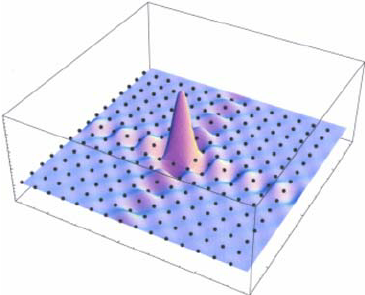
\includegraphics[width=0.5\textwidth]{psinc}
%\caption{An illustration of the periodic cardinal sin function (psinc) basis set used to expand the NGWFs in ONETEP.\cite{psinc}}
%\end{figure}
%
To achieve linear-scaling, it is not efficient to work in terms of the aforementioned electron density ($n(\mathbf{r})$) from the Kohn-Sham equations, and instead formulate the problem in terms of a density matrix defined by (Eq.~\ref{densitymatrix}), where ($f_n$) is the occupancy and ($\psi$) the KS orbitals. It has the property of idempotency ($\rho^2 = \rho$), the electron density can be computed as its diagonal elements ($n(\mathbf{r}) = 2 \rho(\mathbf{r, r'})$) and the total energy of a system is defined as ($E = 2\mathrm{Tr} (\rho H)$).
%
\begin{equation} \label{densitymatrix}
\rho(\mathbf{r, r'}) = \sum_n f_n \psi_n(\mathbf{r}) \psi_n^*(\mathbf{r'})
\end{equation} 
%
Specifically within ONETEP, the density matrix is given in terms of non-orthogonal generalised Wannier functions (NGWFs) that are localised in real space,\cite{psinc} and defined by (Eq.~\ref{ngwf}). The density kernel ($K^{\alpha \beta}$) is a representation of ($f_n$) (Eq.~\ref{densitymatrix}) and must be sparse, so that elements of the NGWF further than a defined cut-off ($r_K$) can be truncated.
%
\begin{equation} \label{ngwf}
\rho(\mathbf{r, r'}) = \sum_{\alpha \beta} \phi_{\alpha} (\mathbf{r}) K^{\alpha \beta} \phi_{\beta}^*(\mathbf{r})
\end{equation}
%
The ground state energy of a given system is then computed by (Eq.~\ref{onetepmin})
%
\begin{equation} \label{onetepmin}
E_0 = \min_n E[n] = \min_\rho E[\rho]_{\rho = \rho^2} = \min_{\mathbf{K}, \phi} E[\mathbf{K}, \phi]
\end{equation}
%
By (Eq.~\ref{onetepmin}), two nested conjugate gradient constrained search loops are used to minimise the total energy. In the outer energy minimisation loop, the density kernel is kept fixed while the energy is minimised with respect to the spatial profile of the NGWFs, which is equivalent to solving a KS eigenvalue problem. In the inner loop, the NGWF expansion is kept fixed while the energy is minimised with respect to the matrix elements of the density kernel. Therefore eventually arriving at a self-consistent Hamiltonian once the right (idempotent) density matrix ($\rho(\mathbf{r, r'})$) is found. %An illustration of an extended eigenstate compared with a localised NGWF is given in figure \ref{fig:oligo}.
%
%\begin{figure}[H]
%\centering
%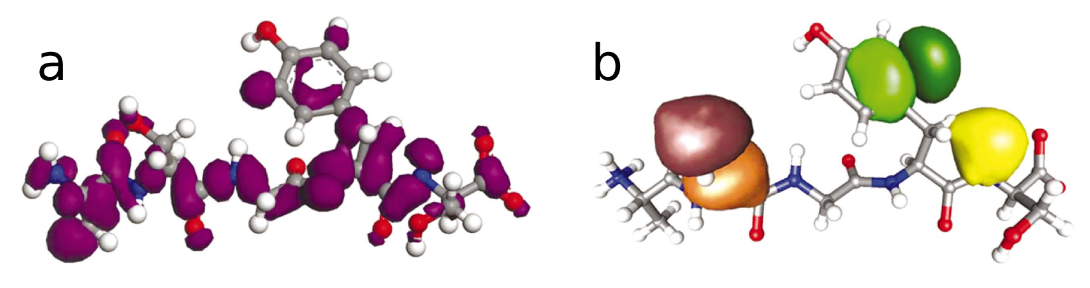
\includegraphics[width=0.99\columnwidth]{ngwf}
%\caption{(a) An extended eigenstate for an oligopeptide molecule, (b) localised NGWFs for the same molecule.\cite{psinc}}
%\label{fig:oligo}
%\end{figure}
%
\subsection{Bespoke non-bonded forcefield parameters}\label{sec:ddec}
%
The Tkatchenko-Scheffler (TS) method is an approach to post process the ground state electronic density --- produced by the DFT calculations as outlined in (section \ref{sec:linear_scaling}) --- to derive the non-bonded forcefield parameters from (Eq.~\ref{eq:forcefield}) for use in MD simulations.\cite{tkatchenko2009accurate} It utilises the charge density dependence of both atomic charges as well as Lennard-Jones parameters, therefore accounting for the impact of the local chemical environment on the van der Waals contributions and point charges of atoms. The TS \edit{method} requires an atoms-in-molecule method, which uses the ground state DFT electronic density of the molecular system ($n(\mathbf{r})$) to divide into uniform overlapping atomic densities ($n_{A}(\mathbf{r})$) through a weighting factor $w_{A}(\mathbf{r})$ (Eq.~\ref{eq:TS}).\cite{tkatchenko2009accurate,manz2012improved}
%
\begin{equation} \label{eq:TS}
n_{A}(\mathbf{r})=w_{A}(\mathbf{r})\,n_{\mathrm{mol}}(\mathbf{r})
\end{equation}
%
The weighting factor is calculated by computing the share of each isolated atom ($n_{A}^0(\mathbf{r})$) of the ($N$) atoms that make up a promolecule ($n_{\mathrm{mol}}^0(\mathbf{r})$). A promolecule is an ideal reference system composed of non-interacting atoms fixed at the same positions in the corresponding molecular system.
\begin{equation}
    n_{\mathrm{mol}}^0(\mathbf{r}) = \sum_{A=1}^N n_{A}^0(\mathbf{r})
\end{equation}
where the weighting factors are differently formulated according to the atoms-in-molecule scheme, in the iterative Hirshfeld (IH) scheme,\cite{bultinck2007uniqueness} it is given by:
\begin{equation}
    w_{A}^{\mathrm{IH}}(\mathbf{r}) = \frac{n_{A}^0(\mathbf{r})}{n_{\mathrm{mol}}^0(\mathbf{r})}
\end{equation}
The self-consistency of the IH scheme therefore requires that the share of the isolated atomic densities ($n_{A}^0(\mathbf{r})$) from the promolecular density ($n_{\mathrm{mol}}^0(\mathbf{r})$) is equivalent to the share of the overlapping atomic density ($n_{A}(\mathbf{r})$) from the total molecular density ($n_{\mathrm{mol}}(\mathbf{r})$). The atomic electron population ($N_A$) are derived from the atomic densities ($n_{A}(\mathbf{r})$) by:
%
\begin{equation}
    N_A = \int n_A (\mathbf{r}) \mathrm{d}\mathbf{r}
\end{equation}
%
In the IH scheme, the isolated atomic density is composed of the weighted average of the atomic densities with the next lowest integer ($\mathrm{lint}(N_A)$) and next highest integer ($\mathrm{uint}(N_A)$) occupancies. %
\begin{equation}
\begin{aligned}
n_{A}^{0, N_{A}}(\mathbf{r})=& \,\,n_{A}^{0, \operatorname{lint}\left(N_{A}\right)}(\mathbf{r})\left[\operatorname{uint}\left(N_{A}\right)-N_{A}\right] \\
&+n_{A}^{0, \operatorname{uint}\left(N_{A}\right)}(\mathbf{r})\left[N_{A}-\operatorname{lint}\left(N_{A}\right)\right]
\end{aligned}
\end{equation}
The weighting factor in the iterated stockholder atoms (ISA) scheme \cite{lillestolen2008redefining} is instead defined with respect to the spherical average of the electronic density around atom ($A$) by (Eq.~\ref{eq:ISA_weights}). Unlike IH, the self-consistency in ISA requires that every value of the radius of a sphere around each nucleus ($A$), the average electron density on the surface of this sphere is the same in the promolecular atom ($\langle n_{A}^{0, \mathrm{ISA}}(d)\rangle$) and in the atom in the molecule ($\langle n_{A}^{\mathrm{ISA}}(d)\rangle$).\cite{bultinck2009comparison}
%
\begin{equation} \label{eq:ISA_weights}
w_{A}^{\mathrm{ISA}}(\mathbf{r})=\frac{\left\langle n_{A}^{0,\mathrm{ISA}}\left(\left|\mathbf{r}-\mathbf{R}_{A}\right|\right)\right\rangle}{n_{\mathrm{mol}}^{0, \mathrm{ISA}}(\mathbf{r})}
\end{equation}
where ($\langle n_{A}^{0, \mathrm{ISA}}\left(\left|\mathbf{r}-\mathbf{R}_{A}\right|\right)\rangle$) is the average density over the surface of a sphere with radius ($d$) for an isolated atom ($A$). The promolecular density in (Eq.~\ref{eq:ISA_weights}) is similarly defined as the sum of spherically averaged spheres of radii ($|\mathbf{r} - \mathbf{R}_B|$) around every atom ($B$):
%
\begin{equation}
n_{\mathrm{mol}}^{0, \mathrm{ISA}}(\mathbf{r})=\sum_{B=1}^{N}\left\langle n_{B}^{0, \mathrm{ISA}}\left(\left|\mathbf{r}-\mathbf{R}_{B}\right|\right)\right\rangle
\end{equation}
The density derived electrostatic and chemical electron density partitioning (DDEC) method is one of the atoms-in-molecule electronic density partitioning approaches. DDEC uses a mixture of both IH and ISA methods and iteratively optimises for a converged solution to the weighing factor to resemble the spherical average of the atomic densities ($n_{A}(\mathbf{r})$) and the density of an isolated reference atom ($n_{A}^0(\mathbf{r})$). The atomic partial charges ($q_A$) for MD are derived from DDEC by (Eq.~\ref{eq:ddec_charge}), where ($Z_A$) is the nuclear charge of atom $A$. 
%
\begin{equation} \label{eq:ddec_charge}
    q_A = Z_A - N_A = Z_A - \int n_A(\mathbf{r}) \, \mathrm{d}^3 \mathbf{r}
\end{equation}
%
Whereas the dispersion ($B_{ij}$) and repulsion ($A_{ij}$) coefficients are derived from the partitioned electronic density by (Eq.~\ref{eq:qube_bij}) and (Eq.~\ref{eq:qube_aij}).\cite{horton2019qubekit}
\vspace{-2mm}
\begin{subequations} 
\begin{align}
\begin{split}\label{eq:qube_bij}
B_{i}=\left(\frac{V_{A}^{\mathrm{DDEC}}}{V_{A}^{\mathrm{free}}}\right)^{2} B_{i}^{\mathrm{free}}
\end{split}\\
\begin{split}\label{eq:qube_aij}
A_{i}=\frac{1}{2} B_{i}\left(2 R_{A}^{\mathrm{DDEC}}\right)^{6}
\end{split}
\end{align}
\end{subequations}
%
The atomic volume ($V_{A}^{\mathrm{DDEC}}$) is calculated from the electronic density:
%
\begin{equation} \label{eq:qube_volume}
V_{A}^{\mathrm{DDEC}}=\int r^{3} n_{A}(\mathbf{r}) \, \mathrm{d}^{3} \mathbf{r}
\end{equation}
%
Whereas the other terms are derived from alternative methods. Namely, the free dispersion coefficients ($B_{i}^{\mathrm{free}}$) are computed using time-dependent DFT calculations of free atoms in vacuum,\cite{chu2004linear} the reference volume ($V_{A}^{\mathrm{free}}$) is calculated using more accurate \textit{ab initio} approaches with explicit treatment of electron correlation effects and the DDEC effective radius of each atom rescales the experimentally derived reference free atom radius ($R_{A}^{\mathrm{free}}$) using (Eq.~\ref{eq:qube_radius}).\cite{horton2019qubekit} 
%
\begin{equation} \label{eq:qube_radius}
R_{A}^{\mathrm{DDEC}}=\left(\frac{V_{A}^{\mathrm{AIM}}}{V_{A}^{\mathrm{free}}}\right)^{1 / 3} R_{A}^{\mathrm{free}}
\end{equation}
%
The dispersion and repulsion coefficients are related to the Lennard-Jones parameters, ($\epsilon$) and ($\sigma$), (Eq.~\ref{eq:forcefield}) via ($A_{ij} = 4 \epsilon_{ij}\,\sigma_{ij}^{12}$) and ($B_{ij} = 4 \epsilon_{ij}\,\sigma_{ij}^{6}$). The resulting parameters are an accurate representation of the chemistry of the molecular system under investigation, since they are exclusively derived from \textit{ab initio} quantum mechanical calculations. As such, computing the non-bonded forcefield parameters using DDEC is a basis for bespoke forcefield parametrisation to bypass the use for transferable forcefields. This approach is implemented for small molecules by software such as QUBEKit.\cite{horton2019qubekit} 

%\newpage
\section{\edit{Dynamical Mean Field Theory}}
%
\edit{Strongly correlated materials --- encompassing many transition metal oxides --- typically have incompletely-filled $d$- or $f$-shells, where the on-site Coulombic interactions are comparable with the band-gap. Electronic correlations in such systems give rise to complex behaviour that can no longer be described by the treatment of a single electron within a system of non-interacting particles. As such, single-electron theories such as the local-density approximation (LDA) in density functional theory (DFT) or Hartree-Fock theory fail to accurately describe their electronic structure.\cite{anisimov2010electronic}}

\edit{Strongly correlated materials embody exotic electronic properties that are technologically advantageous or have evolved to be utilised by nature for biological function.\cite{al2020superexchange, weber13, Weber2014a} A study of the Hemocyanin protein core in Chapter requires such a treatment, where extensions to DFT methods are necessary to accurately describe the electronic structure of the strongly correlated metalloprotein active site.\cite{al2020superexchange}}
%
\subsection{\edit{Hubbard model}}
%
\edit{The Hubbard model is a lattice model that describes the interaction of particles of opposite spin on a lattice with sites ($i,j$) through on-site electronic repulsion ($U$) and off-site kinetic hopping ($t$) terms.\cite{kanamori1963electron, hubbard1963electron, gutzwiller1963effect} The Hubbard model Hamiltonian (Eq.~\ref{eq:hubbard_model}) is defined with respect to the creation ($c^{\dagger}$) and annihilation ($c$) operators, for spin indices ($\sigma$) and the occupation of the $i$-th site ($n_i$), where $n_{i \sigma} = c_{i \sigma}^{\dagger} c_{j \sigma}$}.\cite{Anisimov1991a}
%
\begin{equation} \label{eq:hubbard_model}
    \hat{H}_{\mathrm{Hubbard}}=t \sum_{\langle i j\rangle \sigma} c_{i \sigma}^{\dagger} c_{j \sigma}+U \sum_{i} n_{i \uparrow} n_{i \downarrow}
\end{equation}

\edit{Despite its simplistic formulation, the Hubbard model --- unlike conventional approaches --- correctly describes the insulating character of Mott insulators by accounting for the strong repulsion between electrons. In the limit of infinite dimensions or lattice coordination number, the Hubbard model is an exact treatment of the local correlations of a strongly correlated system.\cite{metzner1989correlated}}

\subsection{\edit{Anderson impurity model}}

\edit{The Anderson impurity model (AIM) is a model Hamiltonian that describes magnetic impurities embedded in a metallic system. It is formulated with respect to the intra-site Coulomb repulsion of the impurity energy levels ($\hat{H}_{\mathrm{loc}}$), a bath of conducting electrons ($\hat{H}_{\mathrm{bath}}$) and the coupling term between the impurity and conduction orbitals ($\hat{H}_{\mathrm{mix}}$).\cite{anderson1961localized}}

\begin{equation} \label{eq:AIM}
{H}_{\mathrm{AIM}}=\overbrace{\sum_{i} \epsilon_{i} a_{i}^{\dagger} a_{i}}^{\hat{H}_{\text {bath}}}+\overbrace{\sum_{i \sigma}\left(V_{i}^{\sigma} c_{\sigma}^{\dagger} a_{i \sigma}+ \mathrm{h . c.} \right)}^{\hat{H}_{\text {mix}}}+\overbrace{U n_{\uparrow} n_{\downarrow}-\mu\left(n_{\uparrow}+n_{\downarrow}\right)}^{\hat{H}_{\mathrm{loc}}}
\end{equation}

\edit{The non-correlated electronic levels ($\epsilon_{i}$) of the bath are defined with respect to bath creation ($a_{i}^{\dagger}$) and annihilation ($a_{i}$) operators. The impurity is described by electrons ($n$) interacting through a Coulomb repulsion ($U$) and a chemical potential ($\mu$). The coupling between the impurity and bath orbitals is described by the hybridisation term ($V_{i}^{\sigma}$).}

\edit{The dynamics of the electrons hopping into and out of the bath are described by the impurity Green's function ($G_{\text{imp}}$) and defined with respect to the hybridisation function ($\Delta (\omega) =\sum_{k}\left|V_{k}\right|^{2} /\left(\omega+\mu-\epsilon_{k}\right) $) and the self energy ($\Sigma (\omega)$) for frequency ($\omega$):}
%
\begin{equation}
    G_{\text {imp }}\left(\omega\right) ^ {-1} = \omega+\mu-\epsilon_{k}- \Delta (\omega) - \Sigma_{imp}\left(\omega\right)
\end{equation}
%
\edit{In dynamical mean-field theory (DMFT),\cite{Georges1996a} the lattice (Hubbard) model can be mapped onto a single impurity model, where the single correlated impurity orbital is embedded in an uncorrelated bath of conduction-band states. This mapping is self-consistent, requiring the impurity Green's function to reproduce the lattice dynamics, as described by the local lattice Green's function ($G_{\text{ii}}$), such that:}
%
\begin{equation}
    G_{\text {imp }}\left(\omega\right) = G_{\text {ii}}\left(\omega\right)
\end{equation}
%
\edit{As well as the self-energy:}
%
\begin{equation}
    \Sigma_{\text {imp }}\left(\omega\right) = \Sigma_{\text {ii}}\left(\omega\right)
\end{equation}
%
\edit{A DMFT calculation is solved through an iterative process where the AIM parameters are chosen such that the model Hamiltonian best describes the physics of the real system in question. As the hybridisation function encapsulates all of the contributions of the bath sites to the physics of the impurity sites, the iterative process converges when the hybridisation function satisfies the self-consistency conditions outlined above.\cite{linscott2020onetep}}

\edit{DMFT is a sophisticated method that includes quantum dynamical effects, and takes into account charge fluctuations, spin fluctuations, and thermal excitations. The DMFT approach is very computationally expensive for studying realistic systems, it is therefore combined with DFT in the form of DFT+DMFT to result in a method that belongs to a broad category of embedding approaches.\cite{Georges1996a,dca_reference_cluster_dmft} The DFT+DMFT method accounts for the limitations of DFT by treating the many-body effects of strongly correlated materials explicitly, while limiting this treatment to the correlated subspace of the $d$- or $f$-electrons, thereby side-stepping the prohibitive scaling of quantum chemistry methods.}